\documentclass[12pt,a4paper]{article}

% ─── Page Layout ───────────────────────────────────────────────────────────────
\usepackage[a4paper, margin=0.8in, headheight=14pt]{geometry}

% ─── Fonts (XeLaTeX) ───────────────────────────────────────────────────────────
\usepackage{fontspec}
\usepackage{unicode-math}
\setmainfont{TeX Gyre Pagella}
\setmonofont[Scale=0.88]{TeX Gyre Cursor}
\setmathfont{Latin Modern Math}

% ─── Packages ──────────────────────────────────────────────────────────────────
\usepackage{xcolor}
\usepackage{colortbl}
\usepackage{titlesec}
\usepackage{enumitem}
\usepackage{tabularx}
\usepackage{booktabs}
\usepackage{array}
\usepackage{amsmath}
\usepackage{tikz}
\usetikzlibrary{shapes.geometric, arrows.meta, positioning, calc, fit, decorations.pathreplacing}
\usepackage{tcolorbox}
\tcbuselibrary{skins, breakable}
\usepackage{hyperref}
\usepackage{fancyhdr}
\usepackage{graphicx}
\usepackage{microtype}
\hyphenpenalty=10000
\exhyphenpenalty=10000
\sloppy
\usepackage{caption}
\usepackage{setspace}
\usepackage{multirow}
\usepackage{tocloft}

% ─── Q&A helper ────────────────────────────────────────────────────────────────
\newcommand{\Q}[1]{\textbf{#1}\par\noindent\ignorespaces}

% ─── Colour Palette ────────────────────────────────────────────────────────────
\definecolor{myred}{RGB}{196,30,58}
\definecolor{mydark}{RGB}{30,30,50}
\definecolor{mygreen}{RGB}{14,120,80}
\definecolor{myteal}{RGB}{0,130,140}
\definecolor{myamber}{RGB}{180,100,0}
\definecolor{mypurple}{RGB}{100,30,160}
\definecolor{mygray}{RGB}{246,247,249}
\definecolor{mgframe}{RGB}{180,185,200}
\definecolor{watermark}{RGB}{145,150,170}
\definecolor{hdrred}{RGB}{250,232,235}
\definecolor{hdrgreen}{RGB}{220,244,233}
\definecolor{hdrteal}{RGB}{220,242,244}
\definecolor{hdramber}{RGB}{253,242,215}
\definecolor{hdrpurple}{RGB}{238,228,255}
\definecolor{hdrgray}{RGB}{238,240,245}
\definecolor{rowalt}{RGB}{250,251,253}

% ─── Section Formatting ────────────────────────────────────────────────────────
\titleformat{\section}
  {\large\bfseries\color{myred}}{\thesection.}{0.5em}{}
  [\vspace{1pt}{\color{myred}\rule{\linewidth}{0.8pt}}]
\titleformat{\subsection}
  {\normalsize\bfseries\color{myteal}}{\thesubsection}{0.5em}{}
\titlespacing*{\section}{0pt}{18pt}{7pt}
\titlespacing*{\subsection}{0pt}{11pt}{4pt}

% ─── Paragraph ─────────────────────────────────────────────────────────────────
\setlength{\parindent}{0pt}
\setlength{\parskip}{4pt}

% ─── TOC Styling ───────────────────────────────────────────────────────────────
\renewcommand{\cfttoctitlefont}{\large\bfseries\color{myred}}
\renewcommand{\cftaftertoctitle}{\par\noindent{\color{myred}\rule{\linewidth}{0.8pt}}}
\setlength{\cftbeforetoctitleskip}{0pt}
\setlength{\cftaftertoctitleskip}{6pt}
\renewcommand{\cftsecfont}{\normalsize\bfseries\color{mydark}}
\renewcommand{\cftsecpagefont}{\normalsize\bfseries\color{mydark}}
\renewcommand{\cftsecleader}{\cftdotfill{\cftdotsep}}
\setlength{\cftbeforesecskip}{7pt}
\renewcommand{\cftsubsecfont}{\small\color{mydark}}
\renewcommand{\cftsubsecpagefont}{\small\color{mydark}}
\setlength{\cftbeforesubsecskip}{3pt}
\setlength{\cftsubsecindent}{1.4em}

% ─── Table helpers ─────────────────────────────────────────────────────────────
\renewcommand{\arraystretch}{1.45}
\setlength{\tabcolsep}{6pt}
\arrayrulecolor{mydark}
\newcolumntype{B}[1]{>{\small\bfseries\raggedright\arraybackslash}m{#1}}
\newcolumntype{Y}{>{\small\raggedright\arraybackslash}X}
\renewcommand{\tabularxcolumn}[1]{m{#1}}

% ─── Header / Footer ───────────────────────────────────────────────────────────
\pagestyle{fancy}
\fancyhf{}
\fancyhead[L]{\small\color{myred}\textbf{PE-EC703A}\;\color{mydark}--- Embedded System}
\fancyhead[R]{\small\color{myteal}\textbf{Module 3 Notes}}
\fancyfoot[C]{\small\color{mydark}\thepage}
\fancyfoot[R]{\small\color{watermark}\textit{\copyright\ Biraj}}
\renewcommand{\headrulewidth}{0.5pt}
\renewcommand{\footrulewidth}{0.3pt}

% ─── Hyperref ──────────────────────────────────────────────────────────────────
\hypersetup{
  colorlinks=true, linkcolor=myteal, urlcolor=myteal,
  pdfauthor={Biraj Sarkar},
  pdftitle={PE-EC703A --- Module 3 Notes}
}

% ─── tcolorbox styles ──────────────────────────────────────────────────────────
\tcbset{
  tikzbox/.style={
    colback=mygray, colframe=mgframe, boxrule=0.6pt, arc=4pt,
    left=8pt, right=8pt, top=6pt, bottom=6pt,
    colbacktitle=mgframe, coltitle=mydark,
    fonttitle=\small\bfseries
  },
  defbox/.style={
    colback=hdrgreen, colframe=mygreen, boxrule=0.8pt, arc=4pt,
    left=9pt, right=9pt, top=6pt, bottom=6pt,
    colbacktitle=mygreen, coltitle=white,
    fonttitle=\small\bfseries
  },
  formulabox/.style={
    colback=hdrteal, colframe=myteal, boxrule=0.8pt, arc=4pt,
    left=9pt, right=9pt, top=7pt, bottom=7pt,
    colbacktitle=myteal, coltitle=white,
    fonttitle=\small\bfseries
  },
  examplebox/.style={
    colback=hdramber, colframe=myamber, boxrule=0.8pt, arc=4pt,
    left=9pt, right=9pt, top=6pt, bottom=6pt,
    colbacktitle=myamber, coltitle=white,
    fonttitle=\small\bfseries
  },
  masonbox/.style={
    colback=hdrpurple, colframe=mypurple, boxrule=0.8pt, arc=4pt,
    left=9pt, right=9pt, top=6pt, bottom=6pt,
    colbacktitle=mypurple, coltitle=white,
    fonttitle=\small\bfseries
  },
  exambox/.style={
    colback=hdrpurple, colframe=mypurple, boxrule=1pt, arc=5pt,
    left=10pt, right=10pt, top=8pt, bottom=8pt,
    colbacktitle=mypurple, coltitle=white,
    fonttitle=\bfseries,
    breakable, title after break={\textbf{Frequently Asked / Viva Questions (contd.)}}}
}
\tcbset{breakable}

% ─── TikZ styles ───────────────────────────────────────────────────────────────
\tikzset{
  block/.style={rectangle, draw=myteal, fill=hdrteal,
    text width=2.4cm, align=center, minimum height=0.95cm,
    font=\small, rounded corners=3pt, line width=0.7pt},
  redblock/.style={rectangle, draw=myred, fill=hdrred,
    text width=2.4cm, align=center, minimum height=0.95cm,
    font=\small, rounded corners=3pt, line width=0.7pt},
  netnode/.style={rectangle, draw=myteal, fill=hdrteal,
    text width=1.5cm, align=center, minimum height=0.8cm,
    font=\small, rounded corners=3pt, line width=0.7pt},
  sumjunc/.style={circle, draw=myamber, fill=hdramber,
    minimum size=0.62cm, font=\small, line width=0.8pt},
  snode/.style={circle, draw=mypurple, fill=hdrpurple,
    minimum size=0.55cm, font=\footnotesize, line width=0.7pt},
  arrow/.style={-Stealth, thick, color=mydark},
  redarrow/.style={-Stealth, thick, color=myred},
  line/.style={thick, color=mydark}
}

% ═══════════════════════════════════════════════════════════════════════════════
\begin{document}
% ═══════════════════════════════════════════════════════════════════════════════

\begin{center}
  {\LARGE\bfseries\color{myred} PE-EC703A --- Embedded System}\\[5pt]
  {\normalsize\color{mydark} Semester VII \quad$\bullet$\quad 3L:0T:0P \quad$\bullet$\quad 3 Credits}\\[3pt]
  {\normalsize\color{myteal}\textbf{Module 3 Exam Notes: I/O Types \& Interrupt Service Mechanism}}\\[3pt]
  {\small\color{mydark} CGEC \;$|$\; B.Tech ECE (2023--27) \;$|$\; \textit{Biraj Sarkar}}
\end{center}
\vspace{2pt}
\noindent{\color{myred}\rule{\linewidth}{1.5pt}}
\vspace{2pt}

\hypersetup{linkcolor=mydark}
\tableofcontents
\hypersetup{linkcolor=myteal}
\newpage

% ===============================================================================
\section{Serial and Parallel Communication Ports}
% ===============================================================================

\begin{tcolorbox}[defbox, title={\textbf{Serial vs.\ Parallel Communication}}]
\textbf{Serial Communication:} Data is transmitted one bit at a time over a single wire (or differential pair). Slower per line but uses fewer wires, suitable for long-distance communication.

\textbf{Parallel Communication:} Multiple bits (e.g., 8 bits) are transmitted simultaneously over multiple wires. Faster but requires more wires; limited to short distances due to skew and crosstalk.
\end{tcolorbox}

\par\noindent
{\renewcommand{\arraystretch}{1.55}%
\begin{tabularx}{\linewidth}{|B{3.0cm}|Y|Y|}
\hline
\textbf{Feature} & \textbf{Serial Port (UART)} & \textbf{Parallel Port} \\
\hline
\textbf{Wires} & 2 (TXD, RXD) minimum & 8+ data lines + control \\
\hline
\textbf{Speed} & Lower (per port) & Higher \\
\hline
\textbf{Distance} & Long range (RS-232, RS-485) & Short (PCB-level, $<$1 m) \\
\hline
\textbf{Cost} & Low (fewer pins, simpler hardware) & Higher \\
\hline
\textbf{Examples} & UART, SPI, I2C, USB & 8051 P0--P3 ports, old printer port \\
\hline
\end{tabularx}}

\subsection{UART (Universal Asynchronous Receiver/Transmitter)}
\begin{itemize}[leftmargin=*, itemsep=3pt]
  \item \textbf{Asynchronous:} No shared clock line --- both devices agree on \textbf{baud rate} beforehand.
  \item \textbf{Frame format:} Start bit (1, low) + Data bits (5--9) + Optional Parity bit + Stop bit(s) (1 or 2, high).
  \item \textbf{Baud rate:} Number of signal changes per second (symbols/second). At 9600 baud, 1 bit = 104 $\mu$s.
  \item \textbf{Wiring:} TXD of device A connects to RXD of device B, and vice versa. Ground is shared.
\end{itemize}

\begin{tcolorbox}[formulabox, title={\textbf{UART Baud Rate Formula (8051)}}]
\[
\text{Baud Rate} = \frac{f_{osc}}{32 \times 12 \times (256 - \text{TH1})}
\quad \text{(Mode 1 or 3, Timer 1 in 8-bit auto-reload)}
\]
For 9600 baud at $f_{osc} = 11.0592\,\text{MHz}$: \quad TH1 = FDH (253)
\end{tcolorbox}

% ===============================================================================
\section{Timer and Counting Devices}
% ===============================================================================

\begin{tcolorbox}[defbox, title={\textbf{Timer / Counter}}]
A \textbf{timer} is a hardware counter that increments on each internal clock pulse (counting time). A \textbf{counter} increments on each external event pulse (e.g., counting RPM or pulses). Both use the same hardware register; the source of the clock selects timer vs.\ counter mode.
\end{tcolorbox}

\subsection{8051 Timer Modes}

The 8051 has two timers (Timer 0 and Timer 1), each configurable in 4 modes via TMOD register:

\par\noindent
{\renewcommand{\arraystretch}{1.55}%
\begin{tabularx}{\linewidth}{|B{2.5cm}|Y|Y|}
\hline
\textbf{Mode} & \textbf{Description} & \textbf{Use} \\
\hline
\textbf{Mode 0} & 13-bit timer/counter (TH + 5 LSBs of TL) & Legacy 8048 compatibility \\
\hline
\textbf{Mode 1} & 16-bit timer/counter (TH:TL = 65536 counts) & Long time delays \\
\hline
\textbf{Mode 2} & 8-bit auto-reload (TL counts, TH is reload value) & Baud rate generation \\
\hline
\textbf{Mode 3} & Two independent 8-bit timers (Timer 0 only) & Dual-purpose timing \\
\hline
\end{tabularx}}

\begin{tcolorbox}[formulabox, title={\textbf{Timer Delay Calculation (8051, Mode 1)}}]
\[
\text{Time delay} = (65536 - \text{Initial Count}) \times \frac{12}{f_{osc}}
\]
Example: For 10 ms delay at 12 MHz: Initial Count $= 65536 - 10000 = 55536 =$ D8F0H
\end{tcolorbox}

% ===============================================================================
\section{Watchdog Timer}
% ===============================================================================

\begin{tcolorbox}[defbox, title={\textbf{Watchdog Timer (WDT)}}]
A \textbf{watchdog timer} is a hardware timer that automatically \textbf{resets the microcontroller} if the software fails to periodically reset (``kick'' or ``pet'') it within a defined time interval. It is used to detect and recover from software deadlocks, infinite loops, or crashes in embedded systems.
\end{tcolorbox}

\subsection{Watchdog Timer Operation}

\begin{tcolorbox}[tikzbox, title={Watchdog Timer Operation Flow}]
\centering
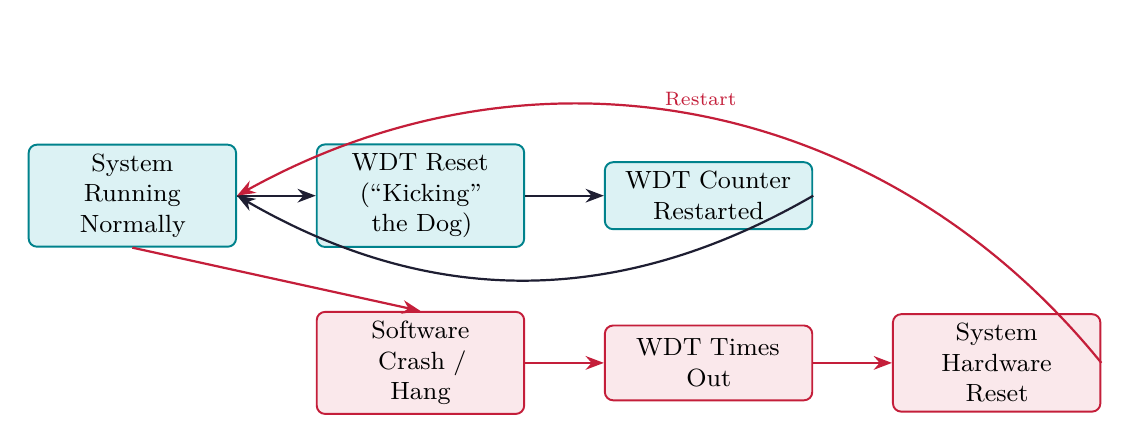
\begin{tikzpicture}[node distance=0.5cm and 1.2cm,
  sblock/.style={rectangle, draw=myteal, fill=hdrteal, text width=2.4cm,
    align=center, minimum height=0.8cm, font=\small, rounded corners=3pt, line width=0.7pt}]
  \node[sblock] (run) {System\\Running\\Normally};
  \node[sblock, right=1.0cm of run] (kick) {WDT Reset\\(``Kicking''\\the Dog)};
  \node[sblock, right=1.0cm of kick] (cnt) {WDT Counter\\Restarted};
  \node[redblock, below=0.8cm of kick] (crash) {Software\\Crash /\\Hang};
  \node[redblock, right=1.0cm of crash] (timeout) {WDT Times\\Out};
  \node[redblock, right=1.0cm of timeout] (reset) {System\\Hardware\\Reset};

  \draw[arrow] (run) -- (kick);
  \draw[arrow] (kick) -- (cnt);
  \draw[arrow] (cnt.east) to[bend left=30] (run.east);
  \draw[redarrow] (run.south) -- (crash.north);
  \draw[redarrow] (crash) -- (timeout);
  \draw[redarrow] (timeout) -- (reset);
  \draw[redarrow] (reset.east) to[bend right=40] node[above, font=\scriptsize\color{myred}] {Restart} (run.east);
\end{tikzpicture}
\end{tcolorbox}

\begin{itemize}[leftmargin=*, itemsep=3pt]
  \item \textbf{Kicking (petting) the WDT:} Software writes a specific value to the WDT register before the timeout period expires. This restarts the countdown.
  \item \textbf{WDT Timeout Period:} Configurable (e.g., 100 ms to several seconds). If not reset in this time, the WDT asserts a hardware reset signal.
  \item \textbf{Window Watchdog (WWDT):} Advanced variant --- must be kicked \textit{within} a specific time window (not too early, not too late) to detect stuck loops that still kick the WDT.
\end{itemize}

% ===============================================================================
\section{Real-Time Clock (RTC)}
% ===============================================================================

\begin{tcolorbox}[defbox, title={\textbf{Real-Time Clock (RTC)}}]
An \textbf{RTC} is a dedicated counter/timer circuit that tracks the current time (hours, minutes, seconds) and date (day, month, year) continuously --- even when the main system is powered off --- using a separate battery (e.g., CR2032 coin cell) and a 32.768 kHz crystal.
\end{tcolorbox}

\begin{itemize}[leftmargin=*, itemsep=3pt]
  \item \textbf{Crystal Frequency:} 32.768 kHz = $2^{15}$ Hz. A 15-bit counter overflows exactly once per second.
  \item \textbf{Interface:} Typically I2C or SPI serial interface (e.g., DS3231, PCF8563).
  \item \textbf{Applications:} Data loggers, digital clocks, alarm systems, access control systems.
  \item \textbf{Alarms/Interrupts:} RTC can generate periodic interrupts (every second, minute, etc.) to wake up the MCU from sleep mode.
\end{itemize}

% ===============================================================================
\section{Serial Bus Communication Protocols}
% ===============================================================================

\subsection{I2C (Inter-Integrated Circuit) Protocol}

\begin{tcolorbox}[defbox, title={\textbf{I2C Protocol}}]
\textbf{I2C} (pronounced ``I-squared-C'') is a synchronous, multi-master, multi-slave, half-duplex serial protocol using only \textbf{two wires}: SDA (Serial Data) and SCL (Serial Clock). Developed by Philips (NXP). Each device has a unique 7-bit (or 10-bit) address.
\end{tcolorbox}

\begin{itemize}[leftmargin=*, itemsep=3pt]
  \item \textbf{Wires:} SDA (bidirectional data) + SCL (clock generated by master). Both are open-drain with pull-up resistors.
  \item \textbf{Speed Modes:} Standard (100 kbps), Fast (400 kbps), Fast-Plus (1 Mbps), High-Speed (3.4 Mbps).
  \item \textbf{Start/Stop Condition:} Start = SDA falls while SCL is high. Stop = SDA rises while SCL is high.
  \item \textbf{ACK/NACK:} After each 8-bit byte, receiver pulls SDA low (ACK) or leaves it high (NACK).
  \item \textbf{Applications:} Connecting sensors (temperature, pressure), EEPROMs, RTC modules, LCD controllers.
\end{itemize}

\begin{tcolorbox}[tikzbox, title={I2C Bus --- Master--Slave Connection}]
\centering
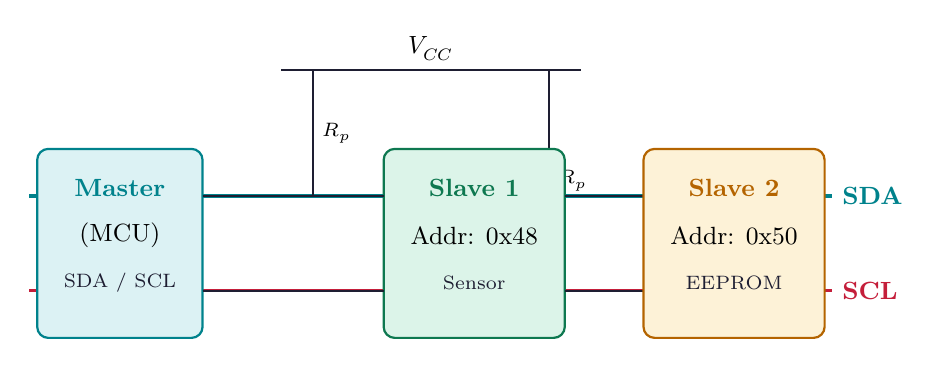
\begin{tikzpicture}[every node/.style={font=\small}, x=1cm, y=1cm]
  % ── Bus lines ──────────────────────────────────────────────────────
  \draw[color=myteal, line width=1.2pt] (0, 2.0) -- (10.2, 2.0);  % SDA
  \draw[color=myred,  line width=1.2pt] (0, 0.8) -- (10.2, 0.8);  % SCL
  \node[right, color=myteal, font=\small\bfseries] at (10.2, 2.0) {SDA};
  \node[right, color=myred,  font=\small\bfseries] at (10.2, 0.8) {SCL};

  % ── VCC rail and pull-ups ──────────────────────────────────────────
  \draw[line width=0.8pt, color=mydark] (3.2, 3.6) -- (7.0, 3.6);   % VCC rail
  \node[above, font=\small] at (5.1, 3.6) {$V_{CC}$};
  % Rp1 on SDA
  \draw[line width=0.8pt, color=mydark] (3.6, 2.0) -- (3.6, 3.6);
  \node[right, font=\scriptsize] at (3.6, 2.8) {$R_p$};
  % Rp2 on SCL
  \draw[line width=0.8pt, color=mydark] (6.6, 0.8) -- (6.6, 3.6);
  \node[right, font=\scriptsize] at (6.6, 2.2) {$R_p$};

  % ── Master ────────────────────────────────────────────────────────
  \draw[fill=hdrteal, draw=myteal, line width=0.8pt, rounded corners=4pt]
    (0.1, 0.2) rectangle (2.2, 2.6);
  \node[font=\small\bfseries, color=myteal]   at (1.15, 2.1) {Master};
  \node[font=\small]                           at (1.15, 1.5) {(MCU)};
  \node[font=\scriptsize, color=mydark]        at (1.15, 0.9) {SDA / SCL};
  % Master connection stubs
  \draw[color=mydark, line width=0.7pt] (2.2, 2.0) -- (3.6, 2.0);
  \draw[color=mydark, line width=0.7pt] (2.2, 0.8) -- (3.6, 0.8);

  % ── Slave 1 ───────────────────────────────────────────────────────
  \draw[fill=hdrgreen, draw=mygreen, line width=0.8pt, rounded corners=4pt]
    (4.5, 0.2) rectangle (6.8, 2.6);
  \node[font=\small\bfseries, color=mygreen] at (5.65, 2.1) {Slave 1};
  \node[font=\small]                          at (5.65, 1.5) {Addr: 0x48};
  \node[font=\scriptsize, color=mydark]       at (5.65, 0.9) {Sensor};
  % Slave 1 connection stubs
  \draw[color=mydark, line width=0.7pt] (4.5, 2.0) -- (3.6, 2.0);
  \draw[color=mydark, line width=0.7pt] (4.5, 0.8) -- (3.6, 0.8);
  \draw[color=mydark, line width=0.7pt] (6.8, 2.0) -- (7.8, 2.0);
  \draw[color=mydark, line width=0.7pt] (6.8, 0.8) -- (7.8, 0.8);

  % ── Slave 2 ───────────────────────────────────────────────────────
  \draw[fill=hdramber, draw=myamber, line width=0.8pt, rounded corners=4pt]
    (7.8, 0.2) rectangle (10.1, 2.6);
  \node[font=\small\bfseries, color=myamber] at (8.95, 2.1) {Slave 2};
  \node[font=\small]                          at (8.95, 1.5) {Addr: 0x50};
  \node[font=\scriptsize, color=mydark]       at (8.95, 0.9) {EEPROM};
  % Slave 2 connection to bus
  \draw[color=mydark, line width=0.7pt] (7.8, 2.0) -- (7.8, 2.0);
  \draw[color=mydark, line width=0.7pt] (7.8, 0.8) -- (7.8, 0.8);
\end{tikzpicture}
\end{tcolorbox}


\subsection{CAN (Controller Area Network) Protocol}

\begin{tcolorbox}[defbox, title={\textbf{CAN Bus Protocol}}]
\textbf{CAN} is a robust, multi-master serial bus protocol designed specifically for \textbf{automotive and industrial} applications where reliability in high-noise environments is critical. It uses differential signaling on two wires: \textbf{CAN-H} (High) and \textbf{CAN-L} (Low). No master/slave --- all nodes are equal.
\end{tcolorbox}

\begin{itemize}[leftmargin=*, itemsep=3pt]
  \item \textbf{Differential Signaling:} CAN-H and CAN-L carry inverted signals. Noise affects both equally and is cancelled at the receiver, giving high EMI immunity.
  \item \textbf{Speed:} Up to 1 Mbps (standard CAN), up to 5--8 Mbps (CAN-FD).
  \item \textbf{Message-Based:} No addresses. Each message has an \textbf{Identifier (ID)} (11-bit or 29-bit). All nodes receive all messages and filter by ID.
  \item \textbf{CSMA/CA:} Carrier Sense Multiple Access with Collision \textbf{Avoidance} --- lower ID (higher priority) wins arbitration without destroying the message.
  \item \textbf{Error Detection:} CRC checking, bit stuffing, ACK slots --- very robust error handling.
  \item \textbf{Applications:} Automotive ECUs, industrial PLCs, medical devices, robotics.
\end{itemize}

\subsection{ISA (Industry Standard Architecture) --- Parallel Bus}

\begin{tcolorbox}[defbox, title={\textbf{ISA Bus}}]
\textbf{ISA} is a \textbf{parallel communication standard} developed by IBM (1981) for connecting peripheral cards (sound cards, modems, I/O cards) to the PC motherboard. It uses an 8-bit or 16-bit wide data bus at 8 MHz. Largely obsolete (replaced by PCI, PCIe) but historically significant.
\end{tcolorbox}

\par\noindent
{\renewcommand{\arraystretch}{1.55}%
\begin{tabularx}{\linewidth}{|B{3.0cm}|Y|Y|Y|}
\hline
\textbf{Feature} & \textbf{I2C} & \textbf{CAN} & \textbf{ISA} \\
\hline
\textbf{Type} & Serial (synchronous) & Serial (async, differential) & Parallel \\
\hline
\textbf{Wires} & 2 (SDA, SCL) & 2 (CAN-H, CAN-L) & 8/16 data + 20 address + control \\
\hline
\textbf{Max Speed} & 3.4 Mbps & 1 Mbps (8 Mbps CAN-FD) & 8 MHz (16 MB/s) \\
\hline
\textbf{Distance} & Short (PCB-level, $<$1 m) & Up to 1 km at 50 kbps & Very short (backplane) \\
\hline
\textbf{Use} & Sensors, EEPROMs & Automotive, industrial & Legacy PC expansion cards \\
\hline
\end{tabularx}}

% ===============================================================================
\section{Interrupt Service Mechanism}
% ===============================================================================

\begin{tcolorbox}[defbox, title={\textbf{Interrupt}}]
An \textbf{interrupt} is a signal sent to the processor by hardware or software indicating that an event requiring immediate attention has occurred. The processor \textbf{suspends} its current task, saves its state (PC, registers), and executes a special routine called the \textbf{Interrupt Service Routine (ISR)}. After the ISR completes, execution resumes from where it was interrupted.
\end{tcolorbox}

\subsection{ISR (Interrupt Service Routine)}

\begin{tcolorbox}[defbox, title={\textbf{ISR --- Interrupt Service Routine}}]
An \textbf{ISR} is a software function that is automatically called by the processor when a specific interrupt occurs. It handles the interrupt event (e.g., reads a received byte from UART, clears a timer flag) and must be kept \textbf{short and fast} to minimize system latency.
\end{tcolorbox}

\begin{tcolorbox}[tikzbox, title={Interrupt Handling Flow}]
\centering
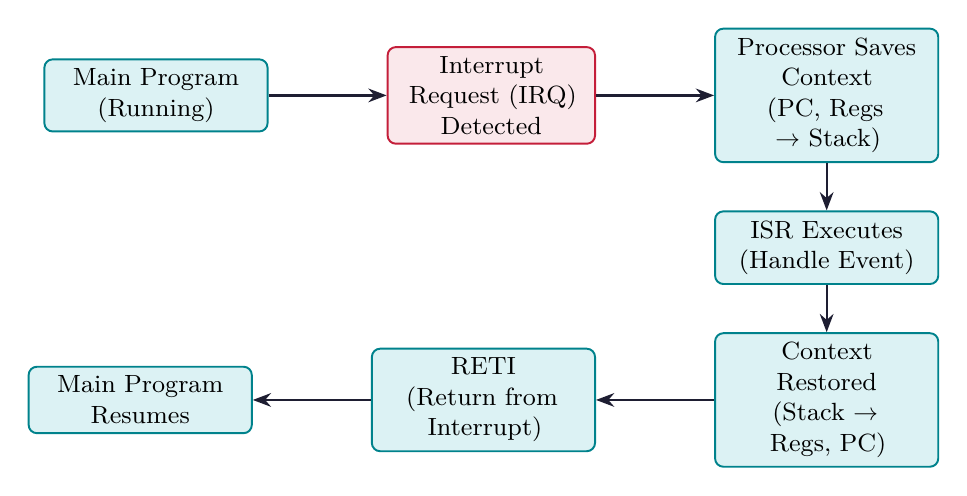
\begin{tikzpicture}[node distance=0.4cm and 1.0cm,
  sblock/.style={rectangle, draw=myteal, fill=hdrteal, text width=2.6cm,
    align=center, minimum height=0.8cm, font=\small, rounded corners=3pt, line width=0.7pt}]
  \node[sblock] (main) {Main Program\\(Running)};
  \node[redblock, right=1.5cm of main] (irq) {Interrupt\\Request (IRQ)\\Detected};
  \node[sblock, right=1.5cm of irq] (save) {Processor Saves\\Context\\(PC, Regs $\to$ Stack)};
  \node[sblock, below=0.6cm of save] (isr) {ISR Executes\\(Handle Event)};
  \node[sblock, below=0.6cm of isr] (rest) {Context\\Restored\\(Stack $\to$ Regs, PC)};
  \node[sblock, left=1.5cm of rest] (ret) {RETI\\(Return from\\Interrupt)};
  \node[sblock, left=1.5cm of ret] (resume) {Main Program\\Resumes};

  \draw[arrow] (main) -- (irq);
  \draw[arrow] (irq) -- (save);
  \draw[arrow] (save) -- (isr);
  \draw[arrow] (isr) -- (rest);
  \draw[arrow] (rest) -- (ret);
  \draw[arrow] (ret) -- (resume);
\end{tikzpicture}
\end{tcolorbox}

\subsection{8051 Interrupt Sources}

The 8051 has \textbf{5 interrupt sources} with a fixed priority:

\par\noindent
{\renewcommand{\arraystretch}{1.55}%
\begin{tabularx}{\linewidth}{|B{3.0cm}|Y|Y|Y|}
\hline
\textbf{Interrupt} & \textbf{Source} & \textbf{Vector Address} & \textbf{Priority (Default)} \\
\hline
\textbf{INT0} & External Pin P3.2 & 0003H & Highest (1) \\
\hline
\textbf{Timer 0} & Timer 0 overflow & 000BH & 2 \\
\hline
\textbf{INT1} & External Pin P3.3 & 0013H & 3 \\
\hline
\textbf{Timer 1} & Timer 1 overflow & 001BH & 4 \\
\hline
\textbf{Serial} & UART TI or RI flag & 0023H & Lowest (5) \\
\hline
\end{tabularx}}

\subsection{Different Interrupt Sources (General)}
\begin{itemize}[leftmargin=*, itemsep=3pt]
  \item \textbf{External Interrupts:} Triggered by a signal change on a pin (edge-triggered or level-triggered).
  \item \textbf{Timer Interrupts:} Triggered when a timer/counter register overflows.
  \item \textbf{Communication Interrupts:} Triggered when UART receives a byte, or SPI transfer completes.
  \item \textbf{ADC Interrupts:} Triggered when analog-to-digital conversion is complete.
  \item \textbf{Software Interrupts (SWI):} Triggered by executing a special instruction (used in ARM for system calls).
  \item \textbf{Reset:} Non-maskable; forces processor to restart (highest priority).
\end{itemize}

% ===============================================================================
\section{Multiple Interrupts, Interrupt Latency and Deadline}
% ===============================================================================

\subsection{Multiple Interrupt Handling}

When several interrupts occur simultaneously, the system must resolve priority:

\begin{itemize}[leftmargin=*, itemsep=3pt]
  \item \textbf{Fixed Priority:} Each interrupt has a fixed, pre-assigned priority level. Higher priority ISR always preempts lower priority (8051 default behavior via IP register).
  \item \textbf{Nested Interrupts:} A higher-priority interrupt can interrupt a currently-executing lower-priority ISR. Requires saving the lower ISR's state on the stack.
  \item \textbf{Interrupt Masking:} Individual interrupts can be enabled/disabled via IE (Interrupt Enable) register bits to prevent interference during critical code sections.
\end{itemize}

\begin{tcolorbox}[masonbox, title={\textbf{8051 Interrupt Enable (IE) Register}}]
\renewcommand{\arraystretch}{1.3}
\begin{tabularx}{\linewidth}{|>{\centering\arraybackslash}X|>{\centering\arraybackslash}X|>{\centering\arraybackslash}X|>{\centering\arraybackslash}X|>{\centering\arraybackslash}X|>{\centering\arraybackslash}X|>{\centering\arraybackslash}X|>{\centering\arraybackslash}X|}
\hline
\textbf{EA} & --- & --- & \textbf{ES} & \textbf{ET1} & \textbf{EX1} & \textbf{ET0} & \textbf{EX0} \\
\hline
Bit 7 & 6 & 5 & 4 & 3 & 2 & 1 & 0 \\
\hline
\end{tabularx}
EA = Global enable; ES = Serial; ET1 = Timer1; EX1 = INT1; ET0 = Timer0; EX0 = INT0
\end{tcolorbox}

\subsection{Interrupt Latency}

\begin{tcolorbox}[defbox, title={\textbf{Interrupt Latency}}]
\textbf{Interrupt latency} is the time elapsed from when an interrupt signal is asserted to when the first instruction of the ISR begins executing. It includes: detecting the interrupt, completing the current instruction, saving context (pushing to stack), and fetching the ISR vector.
\end{tcolorbox}

\begin{tcolorbox}[formulabox, title={\textbf{Interrupt Latency Components}}]
\[
t_{latency} = t_{detect} + t_{inst\_complete} + t_{context\_save} + t_{vector\_fetch}
\]
\begin{itemize}[leftmargin=*, itemsep=2pt, topsep=4pt]
  \item $t_{detect}$: Time for hardware to sample and recognize the interrupt signal.
  \item $t_{inst\_complete}$: Time to finish the currently executing instruction (worst case: longest instruction).
  \item $t_{context\_save}$: Time to push PC (and registers, if applicable) to stack.
  \item $t_{vector\_fetch}$: Time to read the ISR address from the vector table and jump.
\end{itemize}
\textbf{ARM Cortex-M:} Typical latency = 12 clock cycles (with zero wait-state memory).
\end{tcolorbox}

\subsection{Interrupt Deadline}

\begin{tcolorbox}[defbox, title={\textbf{Interrupt Deadline}}]
An \textbf{interrupt deadline} is the maximum allowable time window within which an interrupt request must be fully serviced. It starts at the moment the interrupt event occurs (trigger) and ends when the required response action is completely finished.
\end{tcolorbox}

\subsubsection{Classification of Interrupt Deadlines}
\begin{itemize}[leftmargin=*, itemsep=3pt]
  \item \textbf{Hard Deadline:} Missing the deadline results in total system failure, physical damage, or safety hazards (e.g., airbag deployment, pacemaker pacing pulse, anti-lock braking systems).
  \item \textbf{Soft Deadline:} Missing the deadline degrades the quality of service (QoS) but does not cause system failure (e.g., dropping a frame in video playback, delaying a UI button highlight).
  \item \textbf{Firm Deadline:} Missing the deadline means the processed data is completely useless, but it does not cause catastrophic damage (e.g., packet arrival in telecommunication where outdated packets are simply discarded).
\end{itemize}

\begin{tcolorbox}[formulabox, title={\textbf{Real-Time Constraint \& Timing Budget}}]
For a system to be real-time compliant, the sum of interrupt latency and the ISR execution time must not exceed the deadline:
\[
t_{\text{latency}} + t_{\text{ISR\_execution}} \leq t_{\text{deadline}}
\]
Where:
\begin{itemize}[leftmargin=*, itemsep=2pt, topsep=4pt]
  \item $t_{\text{latency}}$: The time taken to detect the interrupt, save context, and jump to the ISR start.
  \item $t_{\text{ISR\_execution}}$: The execution time of the active instructions inside the ISR.
  \item $t_{\text{deadline}}$: The timing budget imposed by the physical process/application.
\end{itemize}
\end{tcolorbox}

\subsubsection{Key Factors Causing Deadline Violations}
\begin{enumerate}[leftmargin=*, itemsep=3pt]
  \item \textbf{Interrupt Nesting \& Blocking:} If a higher-priority interrupt preempts the current ISR, or if interrupts are globally disabled (during critical sections of the OS), the execution of the lower-priority ISR is delayed, increasing its response time.
  \item \textbf{Interrupt Jitter:} The variance in interrupt latency caused by processor states (pipeline stalls, cache misses, branch mispredictions, or instruction execution state).
  \item \textbf{Over-complex ISRs:} Performing heavy math (e.g., floating-point computations, FFT) or blocking calls (e.g., waiting for serial I/O or delays) inside the ISR.
\end{enumerate}

\subsubsection{Design Strategies to Meet Deadlines}
\begin{itemize}[leftmargin=*, itemsep=3pt]
  \item \textbf{Keep ISRs ``Short and Sweet'':} Perform only the bare minimum operations (e.g., reading a register, clearing a flag, placing data in a circular buffer) and signal the main loop or a background task using a volatile flag or RTOS semaphore.
  \item \textbf{Deferred Processing (Bottom Half):} Defer the heavy non-critical execution to the background (often called a deferred procedure call, tasklet, or thread).
  \item \textbf{Proper Priority Assignment:} Use \textbf{Deadline Monotonic Scheduling (DMS)}, where interrupts with shorter deadlines are assigned higher priority, regardless of their arrival rate.
\end{itemize}

% ===============================================================================
% MANDATORY QUICK REVISION PAGE
% ===============================================================================
\newpage
\begin{center}
  {\large\bfseries\color{myred} Quick Revision --- Module 3}\\[3pt]
  {\small\color{mydark} I/O Types \& Interrupt Service Mechanism $|$ PE-EC703A}
\end{center}
\noindent{\color{myred}\rule{\linewidth}{1.2pt}}
\vspace{4pt}

\begin{tcolorbox}[formulabox, title={\textbf{Key Formulas at a Glance}}]
\renewcommand{\arraystretch}{1.3}
\begin{tabularx}{\linewidth}{B{4.5cm} X}
UART Baud Rate (8051) & $\text{Baud} = \displaystyle\frac{f_{osc}}{32 \times 12 \times (256 - \text{TH1})}$ \\[4pt]
Timer Delay (Mode 1) & $t_{delay} = (65536 - \text{Init\_Count}) \times \displaystyle\frac{12}{f_{osc}}$ \\[4pt]
Interrupt Deadline & $t_{latency} + t_{ISR} \leq t_{deadline}$ \\[4pt]
RTC Crystal Freq & $f = 32768\,\text{Hz} = 2^{15}\,\text{Hz}$ (15-bit counter, 1 overflow/second)
\end{tabularx}
\end{tcolorbox}

\begin{tcolorbox}[defbox, title={\textbf{One-Line Definitions}}]
\begin{itemize}[leftmargin=*, itemsep=2.5pt, topsep=0pt]
  \item \textbf{UART:} Asynchronous serial protocol using start/stop bits; configurable baud rate.
  \item \textbf{I2C:} 2-wire synchronous serial bus (SDA + SCL); multi-master, 7-bit addressing.
  \item \textbf{CAN:} 2-wire differential serial bus for automotive/industrial; message-ID arbitration.
  \item \textbf{ISA:} Legacy 8/16-bit parallel expansion bus from IBM PC (1981); obsolete.
  \item \textbf{Timer:} Hardware counter that counts internal clock pulses to measure time.
  \item \textbf{Counter:} Hardware timer counting external event pulses.
  \item \textbf{WDT:} Watchdog Timer --- resets MCU if software fails to kick it periodically.
  \item \textbf{RTC:} Real-Time Clock --- tracks date and time using 32.768 kHz crystal and coin-cell battery.
  \item \textbf{Interrupt:} Hardware/software signal that suspends main program to run ISR.
  \item \textbf{ISR:} Interrupt Service Routine --- short function handling the interrupt event.
  \item \textbf{Interrupt Latency:} Delay from interrupt request to first ISR instruction.
  \item \textbf{Interrupt Deadline:} Maximum allowable time for ISR to complete its response.
  \item \textbf{NVIC:} ARM's Nested Vectored Interrupt Controller; handles up to 240 priority-based interrupts.
\end{itemize}
\end{tcolorbox}

\begin{tcolorbox}[exambox, title={\textbf{Frequently Asked / Viva Questions}}]
\begin{enumerate}[topsep=0pt, label=\textbf{Q\arabic*.}, itemsep=5pt]
  \item \Q{What is the difference between serial and parallel communication?}
    Serial sends data one bit at a time (fewer wires, longer distance). Parallel sends multiple bits simultaneously (more wires, faster but short-distance only).
  \item \Q{What is UART? Describe its frame format.}
    UART is Universal Asynchronous Receiver/Transmitter. Frame: \textbf{Start bit} (1 bit, low) + \textbf{Data} (5--9 bits, LSB first) + \textbf{Parity bit} (optional) + \textbf{Stop bit(s)} (1 or 2 bits, high). Both ends agree on baud rate; no clock wire.
  \item \Q{What are the two wires in I2C and what do they do?}
    \textbf{SDA} (Serial Data Line): carries data bidirectionally. \textbf{SCL} (Serial Clock Line): carries the synchronization clock generated by the master. Both are open-drain with pull-up resistors.
  \item \Q{Why is CAN used in automobiles instead of I2C or UART?}
    CAN uses differential signaling which is immune to electromagnetic noise. It supports multi-master arbitration (priority-based, non-destructive), reliable error detection (CRC, ACK, bit stuffing), and distances up to 1 km at 50 kbps --- all essential in a noisy vehicle environment.
  \item \Q{What is a Watchdog Timer? Why is it important?}
    A WDT is a hardware timer that resets the MCU if software fails to periodically reset it. It is critical in embedded systems because it provides autonomous recovery from software hangs, infinite loops, or crashes --- without human intervention.
  \item \Q{What is the purpose of the 32.768 kHz crystal in an RTC?}
    32.768 kHz $= 2^{15}$ Hz. A 15-bit counter driven at this frequency overflows exactly once every second, providing a precise 1-second tick for timekeeping without complex division logic.
  \item \Q{Define interrupt latency and list its components.}
    Interrupt latency is the time from interrupt assertion to ISR start. Components: interrupt detection time + current instruction completion time + context save time (PC/regs to stack) + vector table fetch time.
  \item \Q{What is a vector table in embedded systems?}
    A vector table is a fixed memory location (e.g., 0x00000000 in ARM) that stores the starting addresses (vectors) of all ISRs. When an interrupt occurs, the CPU reads the corresponding vector and jumps to the ISR.
  \item \Q{How does the 8051 handle two simultaneous interrupts?}
    The 8051 uses a fixed priority scheme. INT0 has the highest priority and Serial has the lowest. If two interrupts occur simultaneously, the higher-priority one is serviced first. Priority can also be adjusted using the IP (Interrupt Priority) register to create two priority levels.
  \item \Q{What is the difference between edge-triggered and level-triggered interrupts?}
    \textbf{Edge-triggered:} ISR fires on signal transition (rising or falling edge). Responds to event occurrence. \textbf{Level-triggered:} ISR fires as long as the signal remains at the active level. The ISR keeps being called until the condition is cleared.
  \item \Q{Why should an ISR be kept as short as possible?}
    Long ISRs increase interrupt latency for other interrupts, can miss deadlines, may cause data loss (e.g., UART buffer overflow), and increase system unpredictability. Heavy processing should be deferred to the main loop using a flag set by the ISR.
  \item \Q{What is the Timer Mode 2 in 8051 and why is it used for baud rate generation?}
    Mode 2 is an 8-bit auto-reload mode where TL counts from the reload value (stored in TH) to 255 and overflows. On overflow, TL is automatically reloaded from TH. This creates a precise, continuous periodic interrupt --- ideal for generating UART baud rates without software intervention.
\end{enumerate}
\end{tcolorbox}

\begin{tcolorbox}[tikzbox, title={Serial Communication Protocols at a Glance}]
\par\noindent
{\renewcommand{\arraystretch}{1.55}%
\begin{tabularx}{\linewidth}{|B{2.5cm}|Y|Y|Y|Y|}
\hline
\textbf{Protocol} & \textbf{Wires} & \textbf{Speed} & \textbf{Masters} & \textbf{Typical Use} \\
\hline
\textbf{UART} & 2 (TX, RX) & 115.2 kbps typical & 1 & Debug console, GPS \\
\hline
\textbf{SPI} & 4 (MOSI, MISO, SCK, CS) & Up to 50 Mbps & 1 & Flash memory, LCD \\
\hline
\textbf{I2C} & 2 (SDA, SCL) & Up to 3.4 Mbps & Multiple & Sensors, EEPROM \\
\hline
\textbf{CAN} & 2 (CAN-H, CAN-L) & Up to 1 Mbps & Multi-master & Automotive ECU \\
\hline
\textbf{USB} & 4 (D+, D--, VCC, GND) & Up to 10 Gbps & 1 host & PC peripherals \\
\hline
\end{tabularx}}
\end{tcolorbox}

\end{document}
